\section{Auswertung}
\label{sec:Auswertung}
\subsection{Bestimmung der Verdampfungswärme bei einem Druck von maximal 1 bar}
Für den Atmosphärendruck wurde $p_0=\qty{0.993(0.001)}{\bar}$ gemessen.
Die sowohl für $p \leq \qty{1}{\bar}$, als auch für $p>\qty{1}{\bar}$ aufgenommenen Werte für $T$ und $p$ wurden in der Tabelle \ref{tab:tabelle1} angeführt.
\begin{table}[htbp]
    \caption{In der Tabelle ist der Druck in Abhängigkeit zur Temperatur eingetragen.}
    \label{tab:tabelle1}
    \begin{minipage}[t]{0.3\linewidth}
    \begin{tblr}[t]{
        colspec={S[table-format=3.0] S[table-format=1.1] S[table-format=1.3] S[table-format=1.3]},
        row{1}={guard, mode=math},
        vline{2}={2}{-}{text=\clap{$\pm$}},
        vline{4}={2}{-}{text=\clap{$\pm$}},
    }
        \toprule
        \SetCell[c=2]{c} T \mathbin{/} \unit{\celsius} & &\SetCell[c=2]{c} p \mathbin{/} \unit{\bar}&\\
        \midrule
        19 & 0.5 &   0.057 & 0.001       \\
        20 & 0.5 &   0.076 & 0.001       \\
        21 & 0.5 &   0.081 & 0.001       \\
        22 & 0.5 &   0.086 & 0.001       \\
        23 & 0.5 &   0.090 & 0.001       \\
        24 & 0.5 &   0.094 & 0.001       \\
        25 & 0.5 &   0.098 & 0.001       \\
        26 & 0.5 &   0.102 & 0.001       \\
        27 & 0.5 &   0.105 & 0.001       \\
        28 & 0.5 &   0.109 & 0.001       \\
        29 & 0.5 &   0.113 & 0.001       \\
        30 & 0.5 &   0.116 & 0.001       \\
        31 & 0.5 &   0.120 & 0.001       \\
        32 & 0.5 &   0.124 & 0.001       \\
        33 & 0.5 &   0.127 & 0.001       \\
        34 & 0.5 &   0.131 & 0.001       \\
        35 & 0.5 &   0.135 & 0.001       \\
        36 & 0.5 &   0.138 & 0.001       \\
        37 & 0.5 &   0.143 & 0.001       \\
        38 & 0.5 &   0.146 & 0.001       \\
        39 & 0.5 &   0.150 & 0.001       \\
        40 & 0.5 &   0.154 & 0.001       \\
        41 & 0.5 &   0.157 & 0.001       \\
        42 & 0.5 &   0.161 & 0.001       \\
        43 & 0.5 &   0.165 & 0.001       \\
        44 & 0.5 &   0.170 & 0.001       \\
        45 & 0.5 &   0.175 & 0.001       \\
        46 & 0.5 &   0.179 & 0.001       \\
        47 & 0.5 &   0.184 & 0.001       \\
        48 & 0.5 &   0.189 & 0.001       \\
        49 & 0.5 &   0.194 & 0.001       \\
        50 & 0.5 &   0.197 & 0.001       \\
        51 & 0.5 &   0.204 & 0.001       \\
        52 & 0.5 &   0.210 & 0.001       \\
        53 & 0.5 &   0.215 & 0.001       \\
        54 & 0.5 &   0.221 & 0.001       \\
        \bottomrule 
    \end{tblr}
\end{minipage}
\hfill
\begin{minipage}[t]{0.3\linewidth}
    \begin{tblr}[t]{
        colspec={S[table-format=3.0] S[table-format=1.1] S[table-format=1.3] S[table-format=1.3]},
        row{1}={guard, mode=math},
        vline{2}={2}{-}{text=\clap{$\pm$}},
        vline{4}={2}{-}{text=\clap{$\pm$}},
    }
        \toprule
        \SetCell[c=2]{c} T \mathbin{/} \unit{\celsius} & &\SetCell[c=2]{c} p \mathbin{/} \unit{\bar}&\\
        \midrule
        55  & 0.5 &   0.226  & 0.001     \\
        56  & 0.5 &   0.231  & 0.001     \\
        57  & 0.5 &   0.238  & 0.001     \\
        58  & 0.5 &   0.246  & 0.001     \\
        59  & 0.5 &   0.251  & 0.001     \\
        60  & 0.5 &   0.257  & 0.001     \\
        61  & 0.5 &   0.263  & 0.001     \\
        62  & 0.5 &   0.268  & 0.001     \\
        63  & 0.5 &   0.278  & 0.001     \\
        64  & 0.5 &   0.285  & 0.001     \\
        65  & 0.5 &   0.293  & 0.001     \\
        66  & 0.5 &   0.301  & 0.001     \\
        67  & 0.5 &   0.311  & 0.001     \\
        68  & 0.5 &   0.320  & 0.001     \\
        69  & 0.5 &   0.328  & 0.001     \\
        70  & 0.5 &   0.340  & 0.001     \\
        71  & 0.5 &   0.349  & 0.001     \\
        72  & 0.5 &   0.361  & 0.001     \\
        73  & 0.5 &   0.373  & 0.001     \\
        74  & 0.5 &   0.386  & 0.001     \\
        75  & 0.5 &   0.400  & 0.001     \\
        76  & 0.5 &   0.416  & 0.001     \\
        77  & 0.5 &   0.434  & 0.001     \\
        78  & 0.5 &   0.450  & 0.001     \\
        79  & 0.5 &   0.469  & 0.001     \\
        80  & 0.5 &   0.488  & 0.001     \\
        81  & 0.5 &   0.505  & 0.001     \\
        82  & 0.5 &   0.524  & 0.001     \\
        83  & 0.5 &   0.545  & 0.001     \\
        84  & 0.5 &   0.564  & 0.001     \\
        85  & 0.5 &   0.587  & 0.001     \\
        86  & 0.5 &   0.605  & 0.001     \\
        87  & 0.5 &   0.627  & 0.001     \\
        88  & 0.5 &   0.641  & 0.001     \\
        89  & 0.5 &   0.656  & 0.001     \\
         \bottomrule 
    \end{tblr}
\end{minipage}
\hfill
\begin{minipage}[t]{0.3\linewidth}
    \begin{tblr}[t]{
        colspec={S[table-format=3.0] S[table-format=1.1] S[table-format=1.3] S[table-format=1.3]},
        row{1}={guard, mode=math},
        vline{2}={2}{-}{text=\clap{$\pm$}},
        vline{4}={2}{-}{text=\clap{$\pm$}},
    }
        \toprule
        \SetCell[c=2]{c} T \mathbin{/} \unit{\celsius} & &\SetCell[c=2]{c} p \mathbin{/} \unit{\bar}&\\
        \midrule
    90  & 0.5 &   0.676  & 0.001     \\
    91  & 0.5 &   0.701    & 0.001   \\
    92  & 0.5 &   0.734    & 0.001   \\
    93  & 0.5 &   0.759    & 0.001   \\
    94  & 0.5 &   0.782    & 0.001   \\
    95  & 0.5 &   0.806    & 0.001   \\
    96  & 0.5 &   0.832    & 0.001   \\
    97  & 0.5 &   0.861    & 0.001   \\
    98  & 0.5 &   0.890    & 0.001   \\
    99  & 0.5 &   0.914    & 0.001   \\
    100 & 0.5 &   0.947    & 0.001   \\
    101 & 0.5 &   0.955    & 0.001   \\
    102 & 0.5 &   0.958    & 0.001   \\
    103 & 0.5 &   0.962    & 0.001   \\
    104 & 0.5 &   0.968    & 0.001   \\
    105 & 0.5 &   0.970    & 0.001   \\
    109 & 0.5 &   0.971    & 0.001   \\
    110 & 0.5 &   0.971    & 0.001   \\
    111 & 0.5 &   0.974    & 0.001   \\
    112 & 0.5 &   0.974    & 0.001   \\
    113 & 0.5 &   0.974    & 0.001   \\
    118 & 0.5 &   1        & 0.001   \\
    131 & 0.5 &   2        & 0.001   \\
    141 & 0.5 &   3        & 0.001   \\
    149 & 0.5 &   4        & 0.001   \\
    156 & 0.5 &   5        & 0.001   \\
    161 & 0.5 &   6        & 0.001   \\
    167 & 0.5 &   7        & 0.001   \\
    172 & 0.5 &   8        & 0.001   \\
    173 & 0.5 &   9        & 0.001   \\
    181 & 0.5 &  10        & 0.001   \\
    186 & 0.5 &  11        & 0.001   \\
    189 & 0.5 &  12        & 0.001   \\
    192 & 0.5 &  13        & 0.001   \\
    195 & 0.5 &  14        & 0.001   \\
    198 & 0.5 &  15        & 0.001   \\
    \bottomrule 
    \end{tblr}
    \end{minipage}
    \hfill
\end{table}

Um einen Mittelwert für die Verdampfungswärme zu bestimmen, wurde die Temperatur in Kelvin umgerechnet und der Kehrwert gebildet.
Für den Druck wurde eine logarithmische Skala gewählt.
Diese Daten wurden in der Abbildung \ref{fig:werte} dargestellt.

\begin{figure}[H]
    \centering
    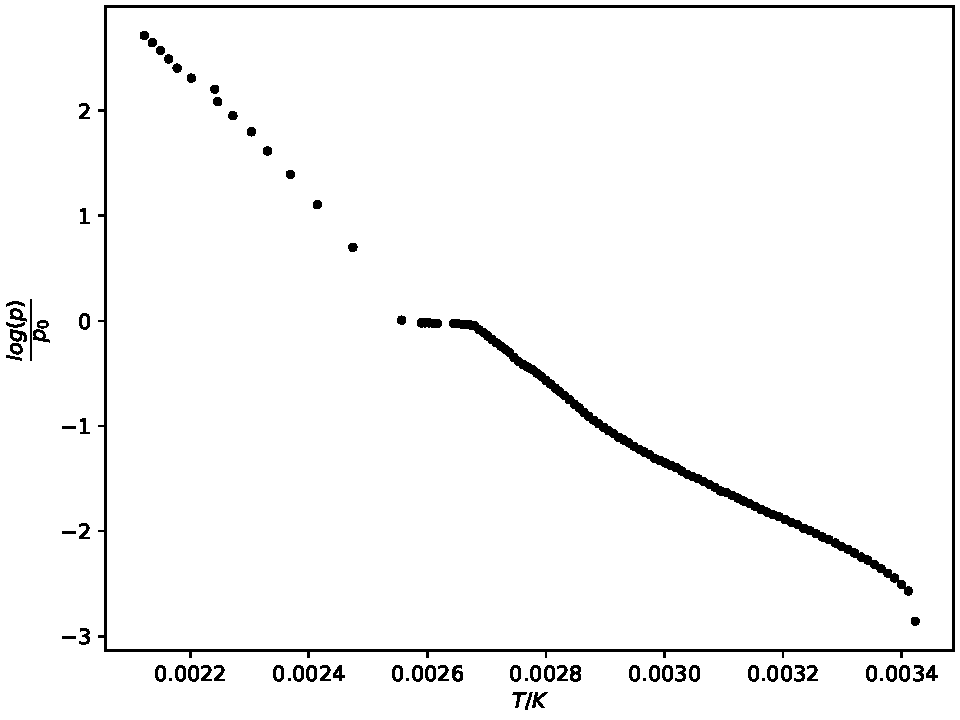
\includegraphics{plot1.pdf}
    \caption{Hier ist der Dampfdruck in Bar auf einer logarithmischen Skala gegen die Temperatur in Kelvin aufgetragen.}
    \label{fig:werte}
\end{figure}

Für den Bereich $p \leq \qty{1}{\bar}$ wurde dann lineare Regression angewandt.
Die in der Abbildung \ref{fig:regression} eingezeichnete Ausgleichsgerade besitzt die Steigung $a=\qty{-3282.759(36.723)}{\kelvin}$.  
Der y-Achsenabschnitt mit $b=\qty{8.6(0.11)}{}$ ist im Gegensatz zu a vernachlässigbar klein.
Diese entspricht $T\.\ln(\frac{p}{p_0})$.
Gleichung \ref{eqn:druck} wird nach der Verdampfungswärme umgestellt und die Steigung der Ausgleichsgeraden wird in 
\begin{equation*}
    L=-R\cdot T\.\ln(\frac{p}{p_0})
\end{equation*}
eingesetzt.
Mit $R=\qty{8.3145}{\joule\per\mole\kelvin}$
Damit ergibt sich $L=\qty{27.3(0.3)e3}{\joule\per\mole}$
\begin{figure}[H]
    \centering
    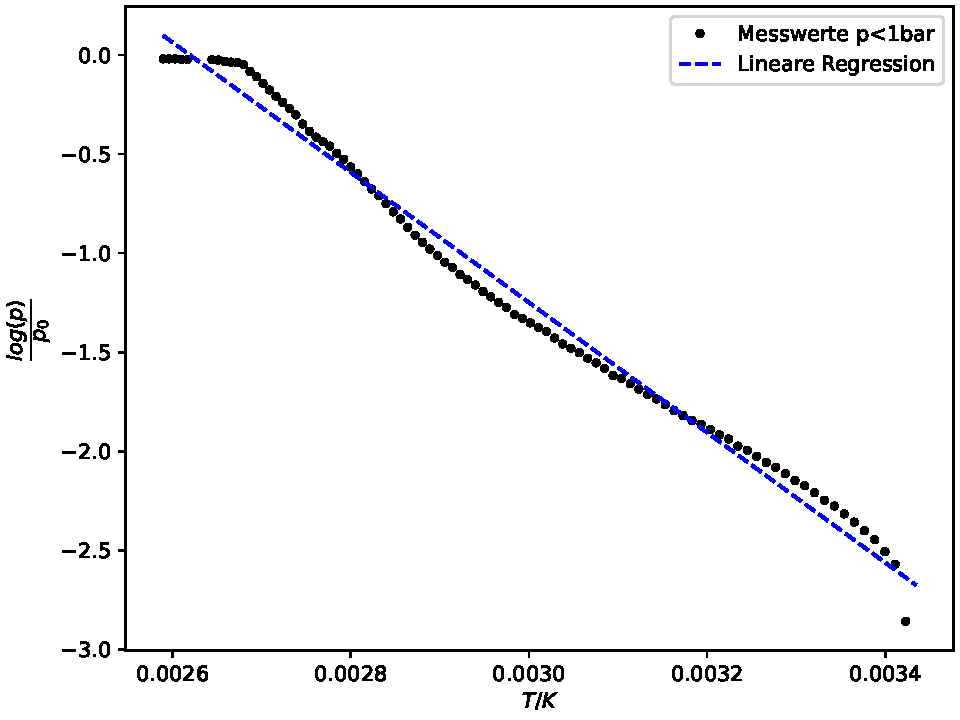
\includegraphics{plot.pdf}
    \caption{Dargestellt ist der Dampfdruck in Bar in logarithmischer Skala, in Abhängigkeit zur Temperatur in Kelvin.
    Zudem wurde eine Ausgleichsgerade eingefügt.}
    \label{fig:regression}
  \end{figure}

\subsection{Bestimmung von der Arbeit um die Anziehungskräfte zwischen Molekülen zu überwinden}
Die Arbeit $L_i$ die benötigt wird, um die intermolekularen Anziehungskräfte zu überwinden, wird mit $L_i=L-L_a$ berechnet.
$L_a$ wird mit $T_a=\qty{373}{\kelvin}$ ausgerechnet.
Es emtspricht $L_a=pV$ und kann in Formel \ref{eqn:gas} eingesetzt werden.
Demnach ist $L_a=RT$ und das entspricht $L_a=\qty{3.1}{\kilo\joule\per\mole}$.
Daraus folgt $L_i=\qty{24.1(0.3)}{\kilo\joule\per\mole}$.
Um die Arbeit für ein einzelnes Molekül zu erhalten, wird $L_I$ durch die Avogradokonstante $N_A=\qty{6.022e23}{\per\mole}$ dividiert.
Umgerechnet in Elektronenvolt ergibt sich $L_i=\qty{0.2501(0.0031)}{eV}$.   


